\documentclass{article}

% if you need to pass options to natbib, use, e.g.:
% \PassOptionsToPackage{numbers, compress}{natbib}
% before loading nips_2018

% ready for submission
% \usepackage{nips_2018}

% to compile a preprint version, e.g., for submission to arXiv, add
% add the [preprint] option:
% \usepackage[preprint]{nips_2018}

% to compile a camera-ready version, add the [final] option, e.g.:
\usepackage[final]{nips_2018}

% to avoid loading the natbib package, add option nonatbib:
% \usepackage[nonatbib]{nips_2018}

\usepackage[utf8]{inputenc} % allow utf-8 input
\usepackage[T1]{fontenc}    % use 8-bit T1 fonts
\usepackage{hyperref}       % hyperlinks
\usepackage{url}            % simple URL typesetting
\usepackage{booktabs}       % professional-quality tables
\usepackage{amsfonts}       % blackboard math symbols
\usepackage{nicefrac}       % compact symbols for 1/2, etc.
\usepackage{microtype}      % microtypography
\usepackage{graphicx}
\title{Deep Learning 2018 - Assignment 1}

% The \author macro works with any number of authors. There are two
% commands used to separate the names and addresses of multiple
% authors: \And and \AND.
%
% Using \And between authors leaves it to LaTeX to determine where to
% break the lines. Using \AND forces a line break at that point. So,
% if LaTeX puts 3 of 4 authors names on the first line, and the last
% on the second line, try using \AND instead of \And before the third
% author name.

\author{
  David Rau (11725184) \\ 
  University of Amsterdam \\
  \texttt{david.rau@student.uva.nl} \\
  %% examples of more authors
  %% \And
  %% Coauthor \\
  %% Affiliation \\
  %% Address \\
  %% \texttt{email} \\
  %% \AND
  %% Coauthor \\
  %% Affiliation \\
  %% Address \\
  %% \texttt{email} \\
  %% \And
  %% Coauthor \\
  %% Affiliation \\
  %% Address \\
  %% \texttt{email} \\
  %% \And
  %% Coauthor \\
  %% Affiliation \\
  %% Address \\
  %% \texttt{email} \\
}

\begin{document}
% \nipsfinalcopy is no longer used

\maketitle


\section*{Vanilla RNN versus LSTM}
\subsection*{Vanilla RNN in PyTorch}
\subsubsection*{Question 1.1}
\subsubsection*{Question 1.3}
The plot that shows the accuracy versus palindrome length of the Vanilla RNN can be found in the answer of Question 1.6.
\subsubsection*{Question 1.4}
\subsection*{Long-Short Term Network (LSTM) in PyTorch}
\subsubsection*{Question 1.5}
\subsubsection*{Question 1.6}
For this exercise the long range dependencies of a simple Vanilla RNN and an LSTM models are probed.  We train on the Palindrome task that is to predict the last character of a symmetric sequence of characters.
The plot that shows the accuracy plotted against the sequence length of both models can be found in Fig. \ref{rnn_lstm_comparison}. Each of the models was trained with the default parameters (learning rate: 0.001, batch size: 128, hidden units: 128, max. steps: 10000) initially. As it can be seen in Fig. \ref{rnn_lstm_comparison} the LSTM with the default learning rate outperforms the Vanilla RNN but the performance collapses from 100\% to around 30\% for sequence length 20. Knowing that LSTMs are, at least in theory, able to keep long distance relationships indefinitely long and that the gradient vanishes with an increasing sequence length, increasing the learning rate should boost the performance. The results show that the LSTM with learning rate 0.01 yields a perfect performance (accuracy 100\%) for all sequence lengths, whereas the Vanilla RNN fails to predict the last character (accuracy $<$ 30\%) from length 11 on.
\begin{figure*}[h!]
    \centering
  \centering
  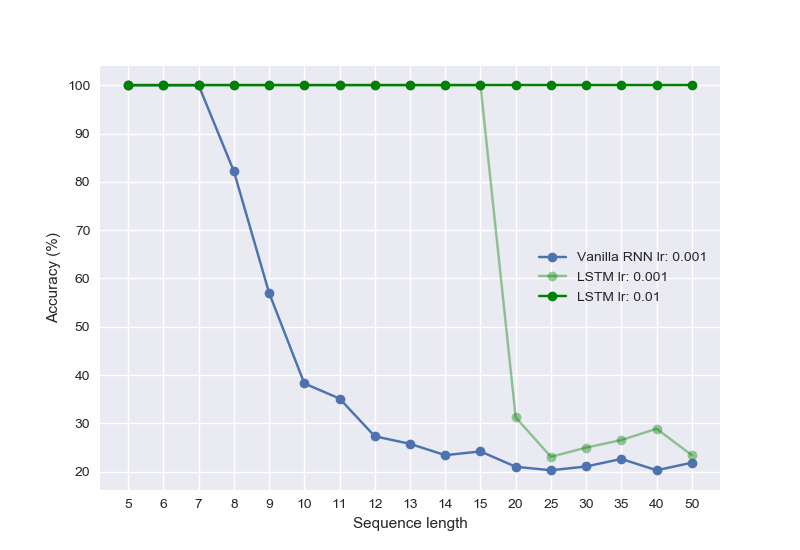
\includegraphics[scale=0.45]{Figure_1}
  \caption{Accuracy (\%) of the Vanilla RNN (blue) and LSTM (green) plotted against different Sequence lengths. The LSTM model was trained with two different learning rates 0.01 and 0.001. }
  \label{rnn_lstm_comparison}
\end{figure*}


\end{document}
